\documentclass[a4paper]{beamer}

\usepackage{polski}
\usepackage[utf8]{inputenc}
\usepackage{amsmath}
\usepackage{amssymb}
\usepackage{enumerate}
\usepackage{hyperref}
\usepackage{listings}
\usepackage{graphicx}
\usepackage{color}

\graphicspath{ {./images/} }
\usetheme{Warsaw}
\useoutertheme{infolines}
\setbeamertemplate{footline}{}
\setbeamertemplate{headline}
{
\begin{beamercolorbox}{section in head/foot}
\vskip2pt\insertnavigation{\paperwidth}\vskip2pt
\end{beamercolorbox}
}

\DeclareGraphicsExtensions{.png}

\author{Agnieszka Pocha \\ Michał Kowalik}
\title{Klątwa wielowymiarowości \\ The Curse of Dimensionality \\ 2. część}
\date{18 marca 2015}

\begin {document}


\begin{frame}
\titlepage
{\footnotesize
na podstawie książki: \\
Bertrand Clarke, Ernest Fokoue, Hao Helen Zhang \\
}
\textit{Principles and Theory for Data Mining and Machine Learning}
\end{frame}


\begin{frame}
\frametitle{Agenda}
\tableofcontents
\end{frame}

\section{Przypomnienie}
\begin{frame}
\begin{block}{Klątwa wielowymiarowości}
Przy wysokim wymiarze przestrzeni, dane są zbyt rzadkie. \\
Przy wysokim wymiarze przestrzeni, liczba możliwych modeli do rozważenia rośnie zbyt szybko.
\end{block}
\end{frame}

\section{Liczba modeli}
\begin{frame}
\begin{block}{}
\textit{In general, the number of polynomial models of order at most $2$ in $p$ variables is $2a - 1$, where $a = 1 + 2p + \frac{p(p-1)}{2}$.}
\end{block}
\begin{block}{Przykład}
Dla $p=1$ jest 7 możliwych różnych modeli: \\
$\mathbb{E}(Y) = \beta_0$, \\
$\mathbb{E}(Y) = \beta_0 + \beta_1 x_1$, \\
$\mathbb{E}(Y) = \beta_0 + \beta_1 x_1 + \beta_2 x_1^2$, \\[0.3cm]


$\mathbb{E}(Y) = \beta_1 x_1$, \\
$\mathbb{E}(Y) = \beta_0 + \beta_2 x_1^2$, \\[0.3cm]


$\mathbb{E}(Y) = \beta_2 x_1^2$, \\
$\mathbb{E}(Y) = \beta_1 x_1 + \beta_2 x_1^2$, \\

\end{block}
\end{frame}

\section{PCA}
\begin{frame}

\begin{block}{Principal Component Analysis - Analiza głównych składowych}
Celem PCA jest taki obrót układu współrzędnych, aby maksymalizować w pierwszej kolejności wariancję pierwszej współrzędnej, następnie wariancję drugiej współrzędnej, itd..
\end{block}

\begin{block}{}
PCA jest często używana do zmniejszania rozmiaru zbioru danych statystycznych, poprzez odrzucenie ostatnich czynników.
\end{block}

\begin{block}{Wariancja}
Klasyczna miara zmienności. Intuicyjnie utożsamiana ze zróżnicowaniem zbiorowości.
$$ D^2(X)=E(X^2)-[E(X)]^2 $$
$E$ - wartość oczekiwana
\end{block}

\end{frame}

\begin{frame}
\begin{block}{Algorytm}
\begin{itemize}
\item Obliczenie wartości średniej dla każdej cechy: $u[m]=\frac{1}{N} \sum\limits_{n=1}^N X[m,n]$
\item Policzenie wartości odchyleń dla każdej komórki danych: $B[i,j] := X'[i,j] =\frac{}{} X[i,j]-u[i]$
\item Wyznaczenie macierzy kowariancji%: $\mathbf{C} = \mathbb{ E } \left[ \mathbf{B} \otimes \mathbf{B} \right] = \mathbb{ E } \left[ \mathbf{B} \cdot \mathbf{B}^{T} \right] = { 1 \over N } \mathbf{B} \cdot \mathbf{B}^{T}$
\item Policzenie wartości własnych macierzy kowariancji \\%: $\mathbf{V}^{-1} \mathbf{C} \mathbf{V} = \mathbf{D} $ \\
{\footnotesize wartość własna opisujące endomorfizm tj. przekształcenie danej przestrzeni liniowej w samą siebie.}
% gdzie $D$ jest macierzą przekątniową wartości własnych $C$.
\item Wybór wartości własnych: można dokonać zawężenia wymiaru przestrzeni.\\
Im wyższa wartość własna tym odpowiadający jej wektor własny jest słabiej skorelowany z pozostałymi.
\item Wyznaczenie wektorów własnych%: $\begin{bmatrix} a_{11}-\lambda & a_{12} \cdots & a_{1n} \\ a_{21} & a_{22}-\lambda \cdots & a_{2n}\\ \vdots & \ddots & \vdots \\ a_{n1} & \cdots & a_{nn}-\lambda\end{bmatrix} \cdot \begin{bmatrix} x_1 \\ x_2 \\ \vdots \\ x_n \end{bmatrix}=0$
\item Rzutowanie na wektory własne%: \\ $y=\begin{bmatrix} y_0 \\ y_1 \\ \vdots \\ y_{n-1} \end{bmatrix}=V^T \cdot x =\begin{bmatrix} v_0^T \\ v_1^T \\ \vdots \\ v_{n-1}^T \end{bmatrix} \cdot x $, gdzie: \\

\end{itemize}
\end{block}
\end{frame}

\section{LDA}
\begin{frame}
\begin{block}{}
LDA
\end{block}
\begin{center}
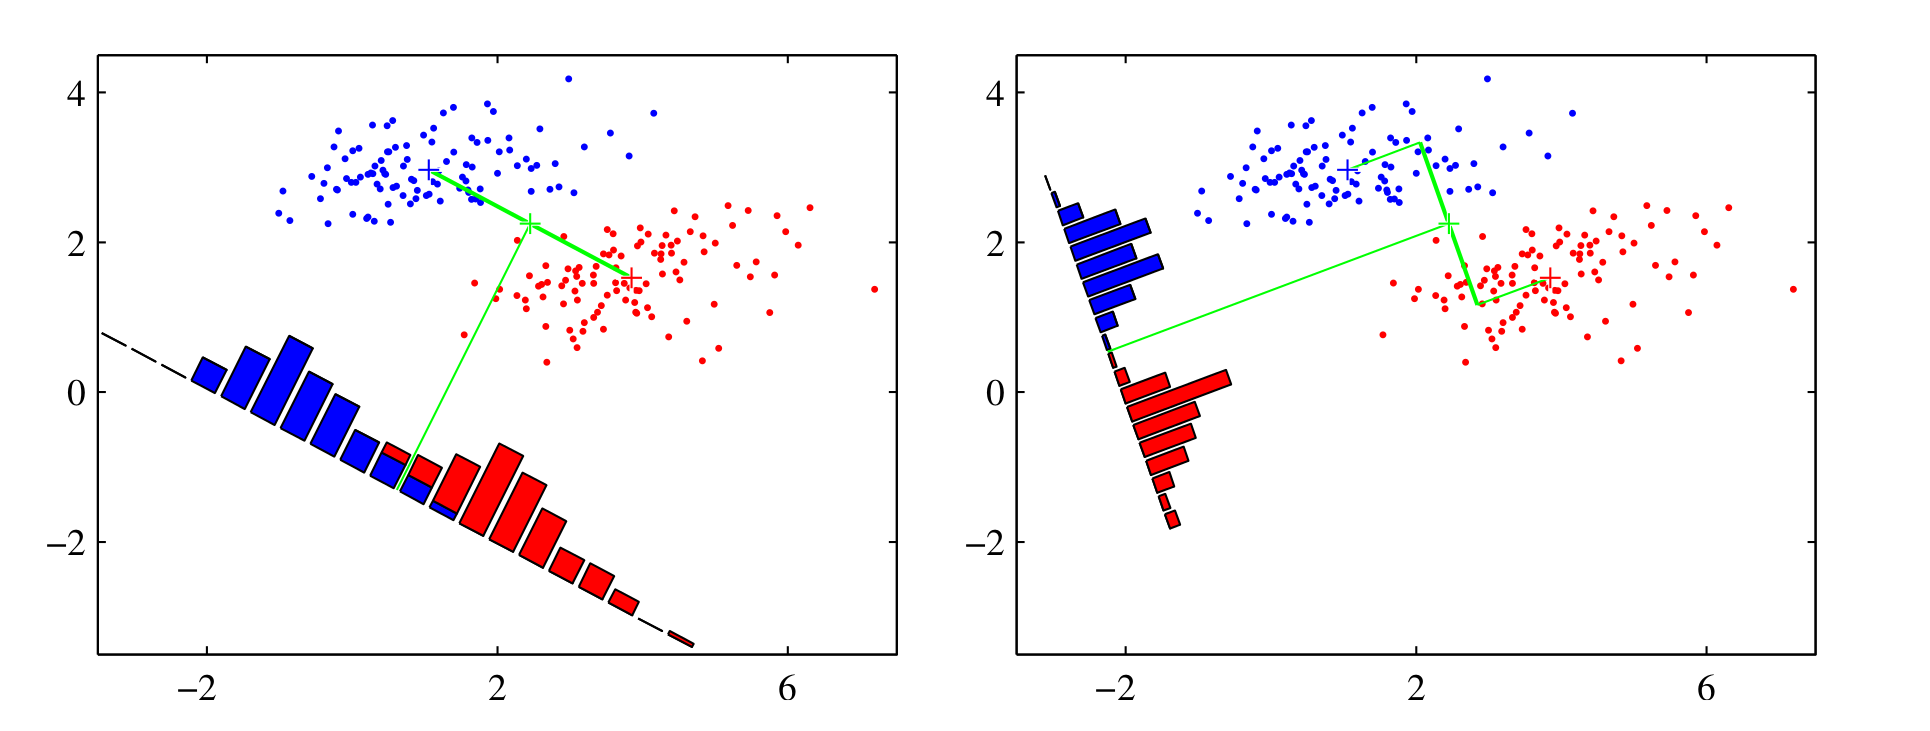
\includegraphics[width=12cm]{bishop-fig4-6.png}
\end{center}
\begin{block}{Przykład}
na modelu: $y = w^T X$
\end{block}
\end{frame}

\begin{frame}
\begin{center}
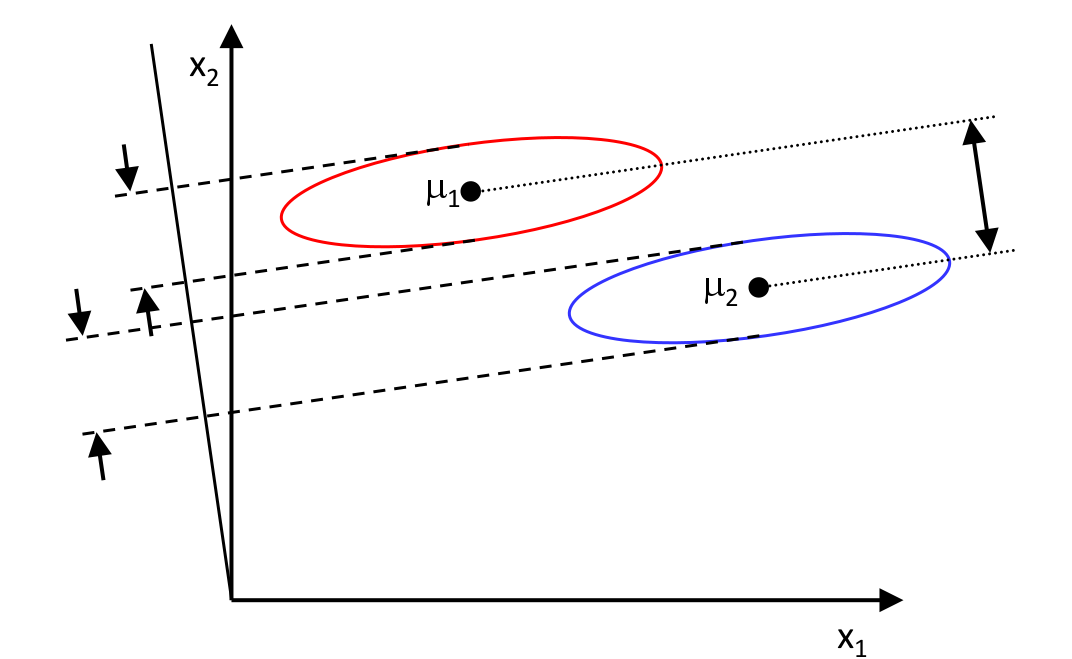
\includegraphics[width=9cm]{fiserNieFukushima.png}
\end{center}
\end{frame}

\section{Model Selection and Assesment}
\begin{frame}
\begin{block}{Wybór Modelu}
oszacowanie jakości róznych modeli w celu wybrania najlepszego. 
\end{block}
\begin{block}{Dopasowanie Modelu}
po wyborze najlepszego modelu, oszacowanie jego błędu przewidywania dla nowych danych.
\end{block}
\pause
\begin{block}{Kryteria}
\begin{itemize}
\item AIC, BIC, Cp - metody analityczne
\item walidacja krzyżowa, Bootstrap - wielokrotne używanie punktów w zbiorach danych.
\end{itemize}
\end{block}
\end{frame}

\section{Cross-validation}
\begin{frame}
\begin{center}
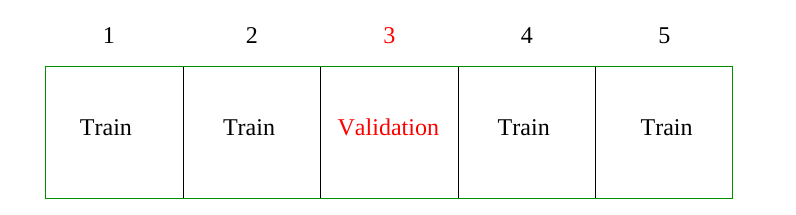
\includegraphics[width=7cm]{corsscalidTibshi.png}
\end{center}
\pause
\begin{center}
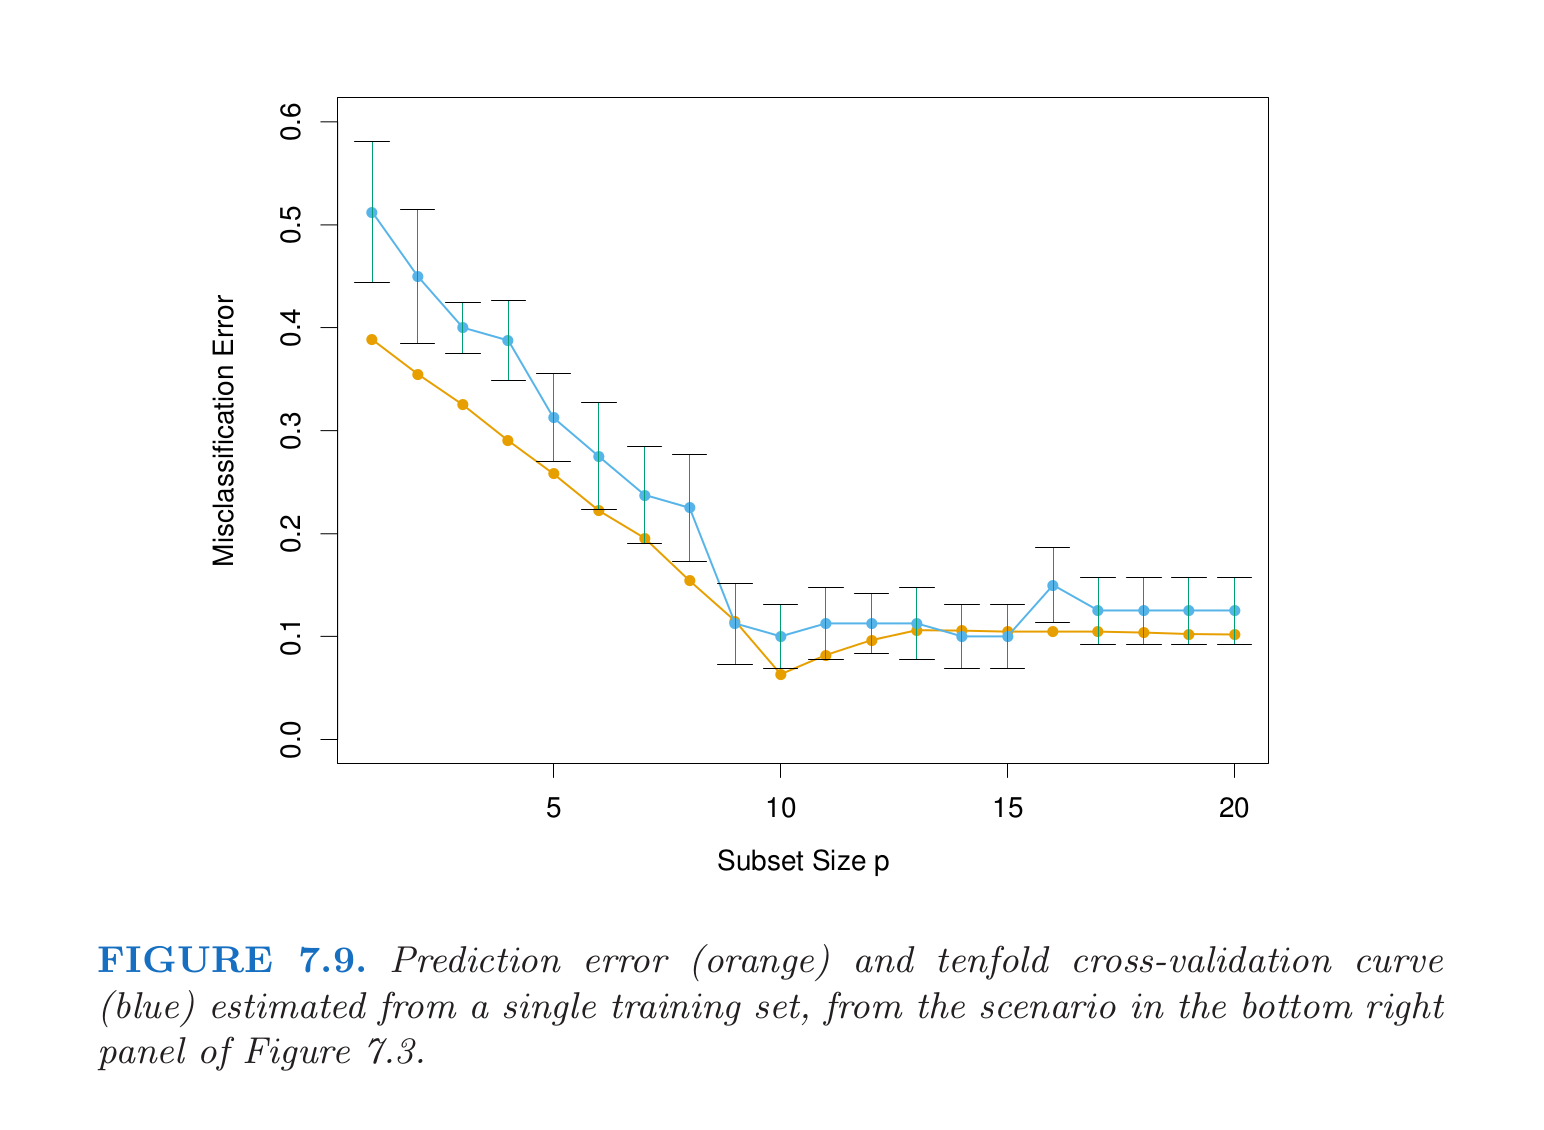
\includegraphics[width=9cm]{fig7-9.png}
\end{center}
\end{frame}

\section{Bootstrap}
\begin{frame}
\begin{block}{Bootstrap}
Bootstrap, to ogólna metoda do oceny statystycznej dokładności.
\end{block}
\begin{block}{}
Główna idea polega na tworzeniu nowych zbiorów poprzez losowanie ze zwracaniem punktów ze zbioru trenującego. Każdy nowy zbiór powinien mieć tę samą wielkość co zbiór trenujący. Tworzy się $B$ nowych zbiorów, następnie dopasowuje się model do każdego z tych nowych zbiorów i sprawdza się jego zachowanie po nauczeniu na każdym z tych nowych zbiorów.
\end{block}
\end{frame}

\begin{frame}

\begin{center}
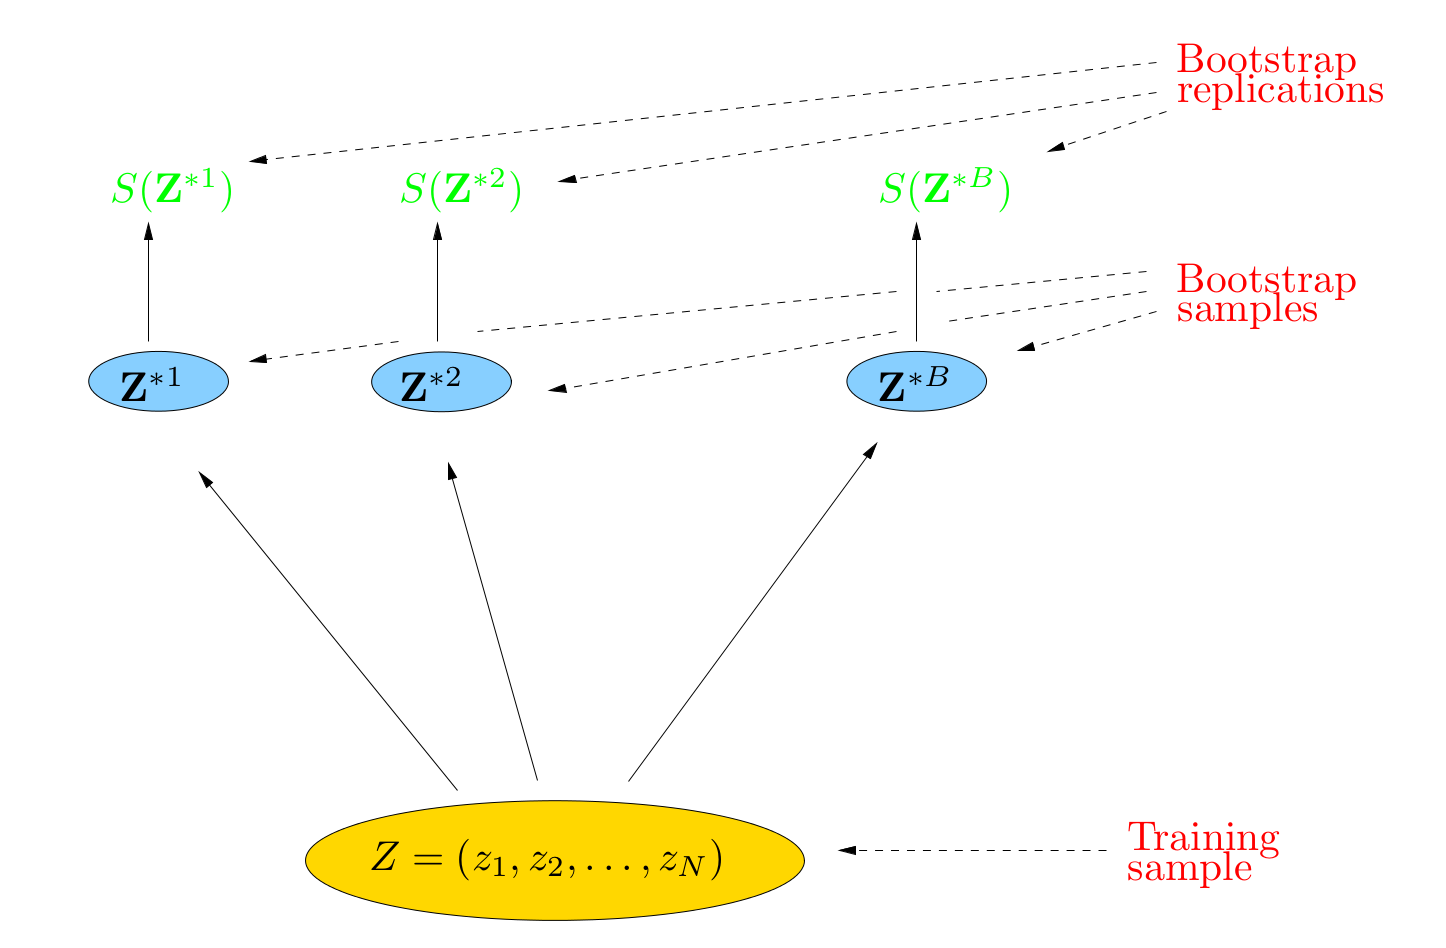
\includegraphics[width=9cm]{fig7-12.png}
\end{center}
\begin{block}{Cel}
Oszacowanie dokładności $S(Z)$ policzonej na podstawie naszego zbioru danych.
\end{block}
\end{frame}

\begin{frame}
\begin{block}{$S(Z)$}
$S(Z)$ - dowolna wartość policzona na podstawie danych $Z$, np. predykcja na podstawie jakiegoś punktu wejściowego.
\end{block}

\begin{block}{}
Na podstawie 'Bootstrap sampling', można oszacować dowolny aspekt dotyczący   rozkładu $S(Z)$.

$$\widehat{Var}[S(Z)] = \frac{1}{B-1} \sum^{B}_{b=1} (S(Z^{* b}) - \tilde{S^{*}})^2$$
gdzie:
$${\text (mean) \ } \tilde{S^{*}} = \frac{1}{B} \sum_b S(Z^{* b})$$
\end{block}
\end{frame}

\begin{frame}
\begin{block}{Jak zaaplikować Bootstrap do oszacowania błędu predykcji?}
Jeśli $\hat{f}^{* b}(x_i)$ to oszacowana wartość w $x_i$ na modelu dopasowanym do $b$-tego nowego zbioru, to szacowana wartość to:
$$\widehat{Err_{boot}} = \frac{1}{B} \frac{1}{N} \sum_{b=1}^{B} \sum_{i=1}^{N} L(y_i, \hat{f}^{* b}(x_i))$$
\end{block}
\pause
\begin{block}{Lepiej}
$$\widehat{Err_{boot}}^{(1)} = \frac{1}{N} \sum^{N}_{i=1} \frac{1}{|C^{-i}|} \sum_{b \in C^{-i}} L (y_i, \hat{f}^{* b}(x_i))$$
\end{block}
\pause
\begin{block}{}
Średnia liczba różnych obserwacji w każdym nowym zbiorze, to około $N \cdot 0.632$.
\end{block}
\end{frame}

\section{AIC}
\begin{frame}
Akaike zaproponował, aby wybierać ten model dla którego najmniejsza jest wartość:
$$\mathrm{AIC}=-2\sum\limits_{j}\ln(\hat{\pi}_j)+2q$$
gdzie: \\
$\hat{\pi}_j$ – estymowane prawdopodobieństwo, przy założeniach danego modelu, uzyskania takiej właśnie wartości obserwacji j jaka była naprawdę uzyskana.\\
$q$ – liczba parametrów modelu
\end{frame}

\section{BIC}
\begin{frame}
Bayesian information criterion (BIC) jest formalnie zdefiniowane jako:
$$\mathrm{BIC} = {-2 \cdot \ln{\hat L} + k \cdot \ln(n)}.$$

gdzie: \\

    $n$ - liczba elementów/przykładów w zbiorze danych \\
    $k$ - Liczba parametrów modelu. \\
    $\hat L$ - Zmaksymalizowana wartość funkcji prawdopodobieństwa dla modelu M

\end{frame}

\section{Vapnik–Chervonenkis dimension}
\begin{frame}
\begin{block}{Vapnik–Chervonenkis (VC) dimension}
Wymiar VC dla klasy $\{f(x, \alpha )\}$ jest zdefiniowane przez najwiekszą liczbę takich punktów (w dowolnej konfiguracji), że można je sklasyfikować przez elementy z $\{f(x, \alpha)\}$.
\end{block}
\begin{block}{Klasyfikowalność zbioru}
Zbiór punktów jest klasyfikowalny przez klasę funkcji jesli, nie ważne jak przyporzadkujemy etykiety binarne do każdego z punktów, istnieje taki element klasy, który może je idealnie separować.
\end{block}
\end{frame}

\begin{frame}
\begin{block}{}
Wymiar VC funkcji liniowych
\end{block}
\begin{center}
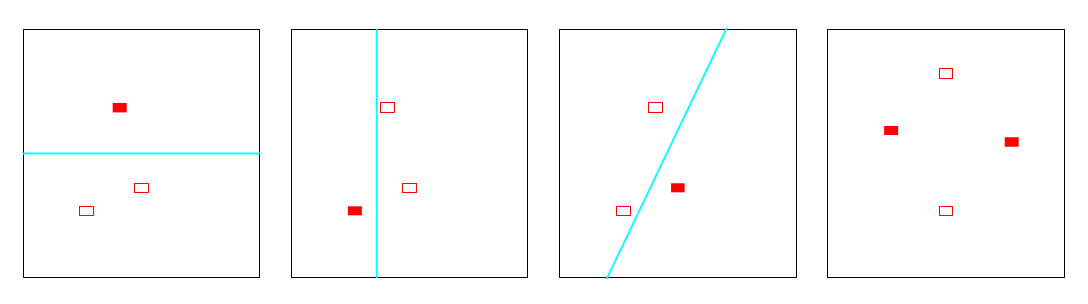
\includegraphics[width=12cm]{fig7-6.png}
\end{center}
\begin{block}{}
W ogóle, liniowy klasyfikator w przestrzeni $p$-wymiarowej ma wymiar VC o rozmiarze $p+1$. \\
Ponadto, można pokazać, że rodzina $\sin(\alpha x)$ ma niekończony wymiar VC. 
\end{block}
\end{frame}

\section{}
\begin{frame}
\begin{block}{}
Często minimalizacja AIC, CV lub Bootstrap wskazuje na model dosyć bliski najlepszego. \\
Jednakże AIC bywa niepraktyczny.
\end{block}
\end{frame}

\end{document}